% Panel (a): physical picture and computational domain.  Canvas ~9 x 6 cm, 10 pt.
\documentclass[12pt,border=2pt,tikz]{standalone}

\usepackage{amsmath}
\usepackage{mhchem}

\newcommand{\GB}{\mathrm{GB}}
\newcommand{\Ox}{\mathrm{O}}

\usetikzlibrary{arrows.meta}

\definecolor{cOx}{RGB}{250,224,80}
\definecolor{cMetal}{RGB}{214,214,211}
\definecolor{cGhost}{RGB}{243,243,241}
\definecolor{cGhostE}{RGB}{168,168,166}
\definecolor{cWater}{RGB}{158,206,232}
\definecolor{cFree}{RGB}{252,252,250}
\definecolor{cEdge}{RGB}{40,40,44}
\definecolor{cAcc}{RGB}{20,72,124}
\definecolor{cRIS}{RGB}{24,104,66}

\begin{document}
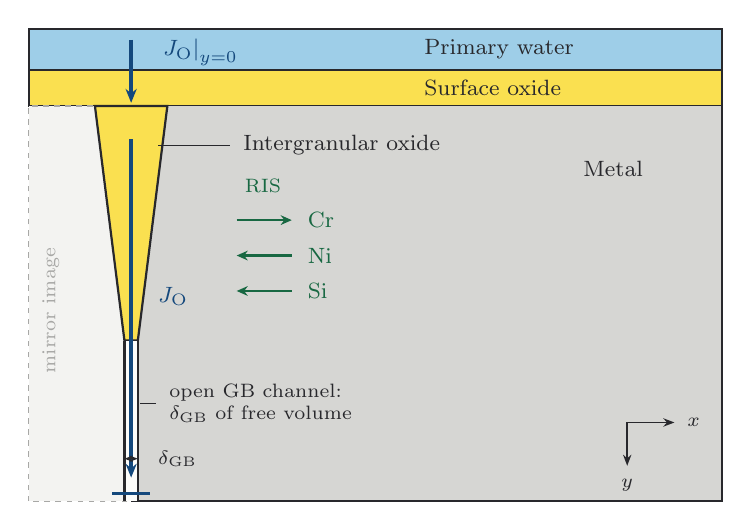
\begin{tikzpicture}[
  x=1cm,y=1cm, font=\footnotesize, color=cEdge,
  eg/.style     ={draw=cEdge,   line width=0.8pt},
  ghosted/.style={draw=cGhostE, line width=0.5pt, dash pattern=on 2pt off 2pt},
  flux/.style   ={-{Stealth[length=5pt,width=4pt]},   line width=1.25pt, draw=cAcc},
  ris/.style    ={-{Stealth[length=4pt,width=3.5pt]}, line width=0.9pt,  draw=cRIS},
  lead/.style   ={draw=cEdge, line width=0.4pt},
]

% ----- geometry --------------------------------------------------------
\def\xL{-1.30}\def\xR{7.50}
\def\yS{2.00}\def\yO{2.46}\def\yW{2.98}
\def\yB{-3.02}
\def\g{0.085}\def\wo{0.46}\def\yf{-0.98}

% ----- water and surface oxide ----------------------------------------
\fill[cWater,eg] (\xL,\yO) rectangle (\xR,\yW);
\fill[cOx  ,eg]  (\xL,\yS) rectangle (\xR,\yO);

% ----- metal: resolved domain (x>0) and a strip of its mirror image ----
\fill[cGhost,ghosted] (\xL,\yB) rectangle (0,\yS);
\fill[cMetal]         (0,\yB)   rectangle (\xR,\yS);
\draw[eg]             (0,\yB) -- (\xR,\yB) -- (\xR,\yS);
\node[cGhostE,font=\scriptsize,rotate=90] at (\xL+0.28,-0.60)
      {mirror image};

% ----- intergranular oxide, and the open GB ahead of it ----------------
\fill[cOx,eg] (-\wo,\yS) -- (\wo,\yS) -- (\g,\yf) -- (-\g,\yf) -- cycle;
\fill[cFree] (-\g,\yB) rectangle (\g,\yf);
\draw[eg] (-\g,\yf) -- (-\g,\yB);
\draw[eg] ( \g,\yf) -- ( \g,\yB);

% ----- oxygen ----------------------------------------------------------
\draw[flux] (0,\yW-0.14) -- (0,\yS+0.04);
\draw[flux] (0,\yS-0.42) -- (0,\yB+0.30);
\draw[cAcc,line width=1.3pt] (-0.24,\yB+0.10) -- (0.24,\yB+0.10);
\node[anchor=west,cAcc] at (0.24,\yW-0.30) {$\left.J_{\Ox}\right|_{y=0}$};
\node[anchor=west,cAcc] at (0.22,-0.42)    {$J_{\Ox}$};

% ----- radiation-induced segregation -----------------------------------
\node[anchor=west,cRIS,font=\scriptsize] at (1.32,0.98) {RIS};
\draw[ris] (1.34,0.55) -- (2.04,0.55);   \node[anchor=west,cRIS] at (2.12,0.55) {Cr};
\draw[ris] (2.04,0.10) -- (1.34,0.10);   \node[anchor=west,cRIS] at (2.12,0.10) {Ni};
\draw[ris] (2.04,-0.35)-- (1.34,-0.35);  \node[anchor=west,cRIS] at (2.12,-0.35){Si};

% ----- labels -----------------------------------------------------------
\node[anchor=west] at (3.60,\yW-0.26) {Primary water};
\node[anchor=west] at (3.60,\yS+0.23) {Surface oxide};
\node[anchor=west] at (5.62,1.20)         {Metal};

\node[anchor=west] at (1.30,1.50) {Intergranular oxide};
\draw[lead] (1.25,1.50) -- (0.34,1.50);

\node[anchor=west,align=left,font=\scriptsize] at (0.36,-1.78)
      {open GB channel:\\ $\delta_{\GB}$ of free volume};
\draw[lead] (0.31,-1.78) -- (\g+0.03,-1.78);
\draw[{Stealth[length=3pt]}-{Stealth[length=3pt]},line width=0.5pt]
      (-\g,-2.48) -- (\g,-2.48);
\node[anchor=west,font=\scriptsize] at (0.22,-2.48) {$\delta_{\GB}$};

% ----- axes -------------------------------------------------------------
\begin{scope}[shift={(6.30,-2.02)}]
  \draw[-{Stealth[length=4pt]},line width=0.7pt] (0,0) -- (0.60,0)
        node[right=1pt,font=\scriptsize] {$x$};
  \draw[-{Stealth[length=4pt]},line width=0.7pt] (0,0) -- (0,-0.55)
        node[below=1pt,font=\scriptsize] {$y$};
\end{scope}

\end{tikzpicture}
\end{document}
